\documentclass[11pt]{article}
\usepackage[margin=1in]{geometry}
\setlength{\parindent}{0pt}
\usepackage{amsmath,amssymb}
\usepackage{graphicx}
\usepackage{caption}
\title{Proposal for a Multi-Arm Biomarker RCT\\Executive Summary}
\author{}
\date{\today}
\begin{document}
\maketitle

Biomarkers are variables that can be measured before treatment that are correlated to treatment outcome. We describe a multi-arm RCT designed to validate treatment-predictive biomarkers in interventional psychiatry. The motivation for this trial is twofold: 
\begin{enumerate}
\item[(1)] Validating biomarkers reported in the literature is more statistically efficient than discovering biomarkers \emph{de novo}, compared to finding biomarkers from scratch.
\item[(2)] Such a trial yields an ideal dataset suitable for finding such novel biomarkers post-hoc. That is, using data from all experimental arms and the combined biomarker data, we fit a predictive model identifying which treatment(s) are most indicated for in an individual patient.
\end{enumerate}

\subsection*{Model and Assumptions}

Consider a trial with \(K\) distinct experimental treatments. A key simplifying assumption we propose is powering for \textbf{one treatment, one biomarker}: each experimental arm \(k\) is assumed indicated by a unique biomarker \(X_k\). This is how biomarkers are reported in the literature (typically linked to a specific intervention) and simplifies the calculations needed to power the trial. In reality, a single biomarker might influence responses to multiple treatments.

\ \\
Formally, the RCT is powered to detect the significance of parameters in the following linear model, relating outcomes \(Y\) for patient index \(i\):

\[
  Y_i \;=\; \beta_0
  \;+\; \sum_{k=1}^K \Bigl[
      \beta_{1k}\,T_{ik}
    \;+\;\beta_{2k}\,X_{ik}
    \;+\;\beta_{3k}\,\bigl(T_{ik} \cdot X_{ik}\bigr)
  \Bigr]
  \;+\;\text{error}_i
\]

where \(T_{ik}\) is the treatment indicator for arm $k$ (binary with \(\sum_k T_{ik}=1\)), and \(X_{ik}\) is the associated biomarker. It's key to interpret the model coefficients in turn:

\medskip
\medskip
\noindent
\begin{tabular}{@{} r p{0.93\textwidth} @{}}
  \(\beta_0\ :\) & The average outcome for the reference treatment group. \\
  \(\beta_{1k}:\) & The main effect of treatment \(k\) compared against the reference treatment. In a traditional RCT, this is the primary estimate under study. \\
  \(\beta_{2k}:\) & The general association of biomarkers with the outcome, irrespective of which treatment the patient received. This accounts for the likely possibility that the biomarker is prognostic for the outcome {\it overall}, which would act as a confounder / nuisance parameter that needs to be controlled for. \\
  \(\beta_{3k}:\) & The \textbf{interaction effect}, which is the \underline{primary} focus of this design. It quantifies how the effect of treatment \(k\) is modulated by its paired biomarker \(X_k\). In this model, the goal for biomarker validation is estimating these interactions accurately, and are hopefully significant. \\
\end{tabular}
\medskip

\subsection*{Power Estimates}

Statistical power is the probability of correctly detecting a true effect when it exists. We performed simulations to estimate power based on plausible biomarker effect sizes, derived from the literature. The biomarkers modeled here comprise EEG measures for rTMS, alcohol use disorder history for ketamine, inflammatory markers for ECT, and speech patterns for novel agents (see main doc for details). These effect estimates are necessarily rough: studies differ among themselves in the population of interest, disease criteria, outcome measures, and the type of statistics reported. We used a conservative procedure (Holm) to control the family-wise error rate, or the probability of making at least one false positive discovery across all \(K\) biomarkers tested.

\begin{figure}[ht!]
\centering
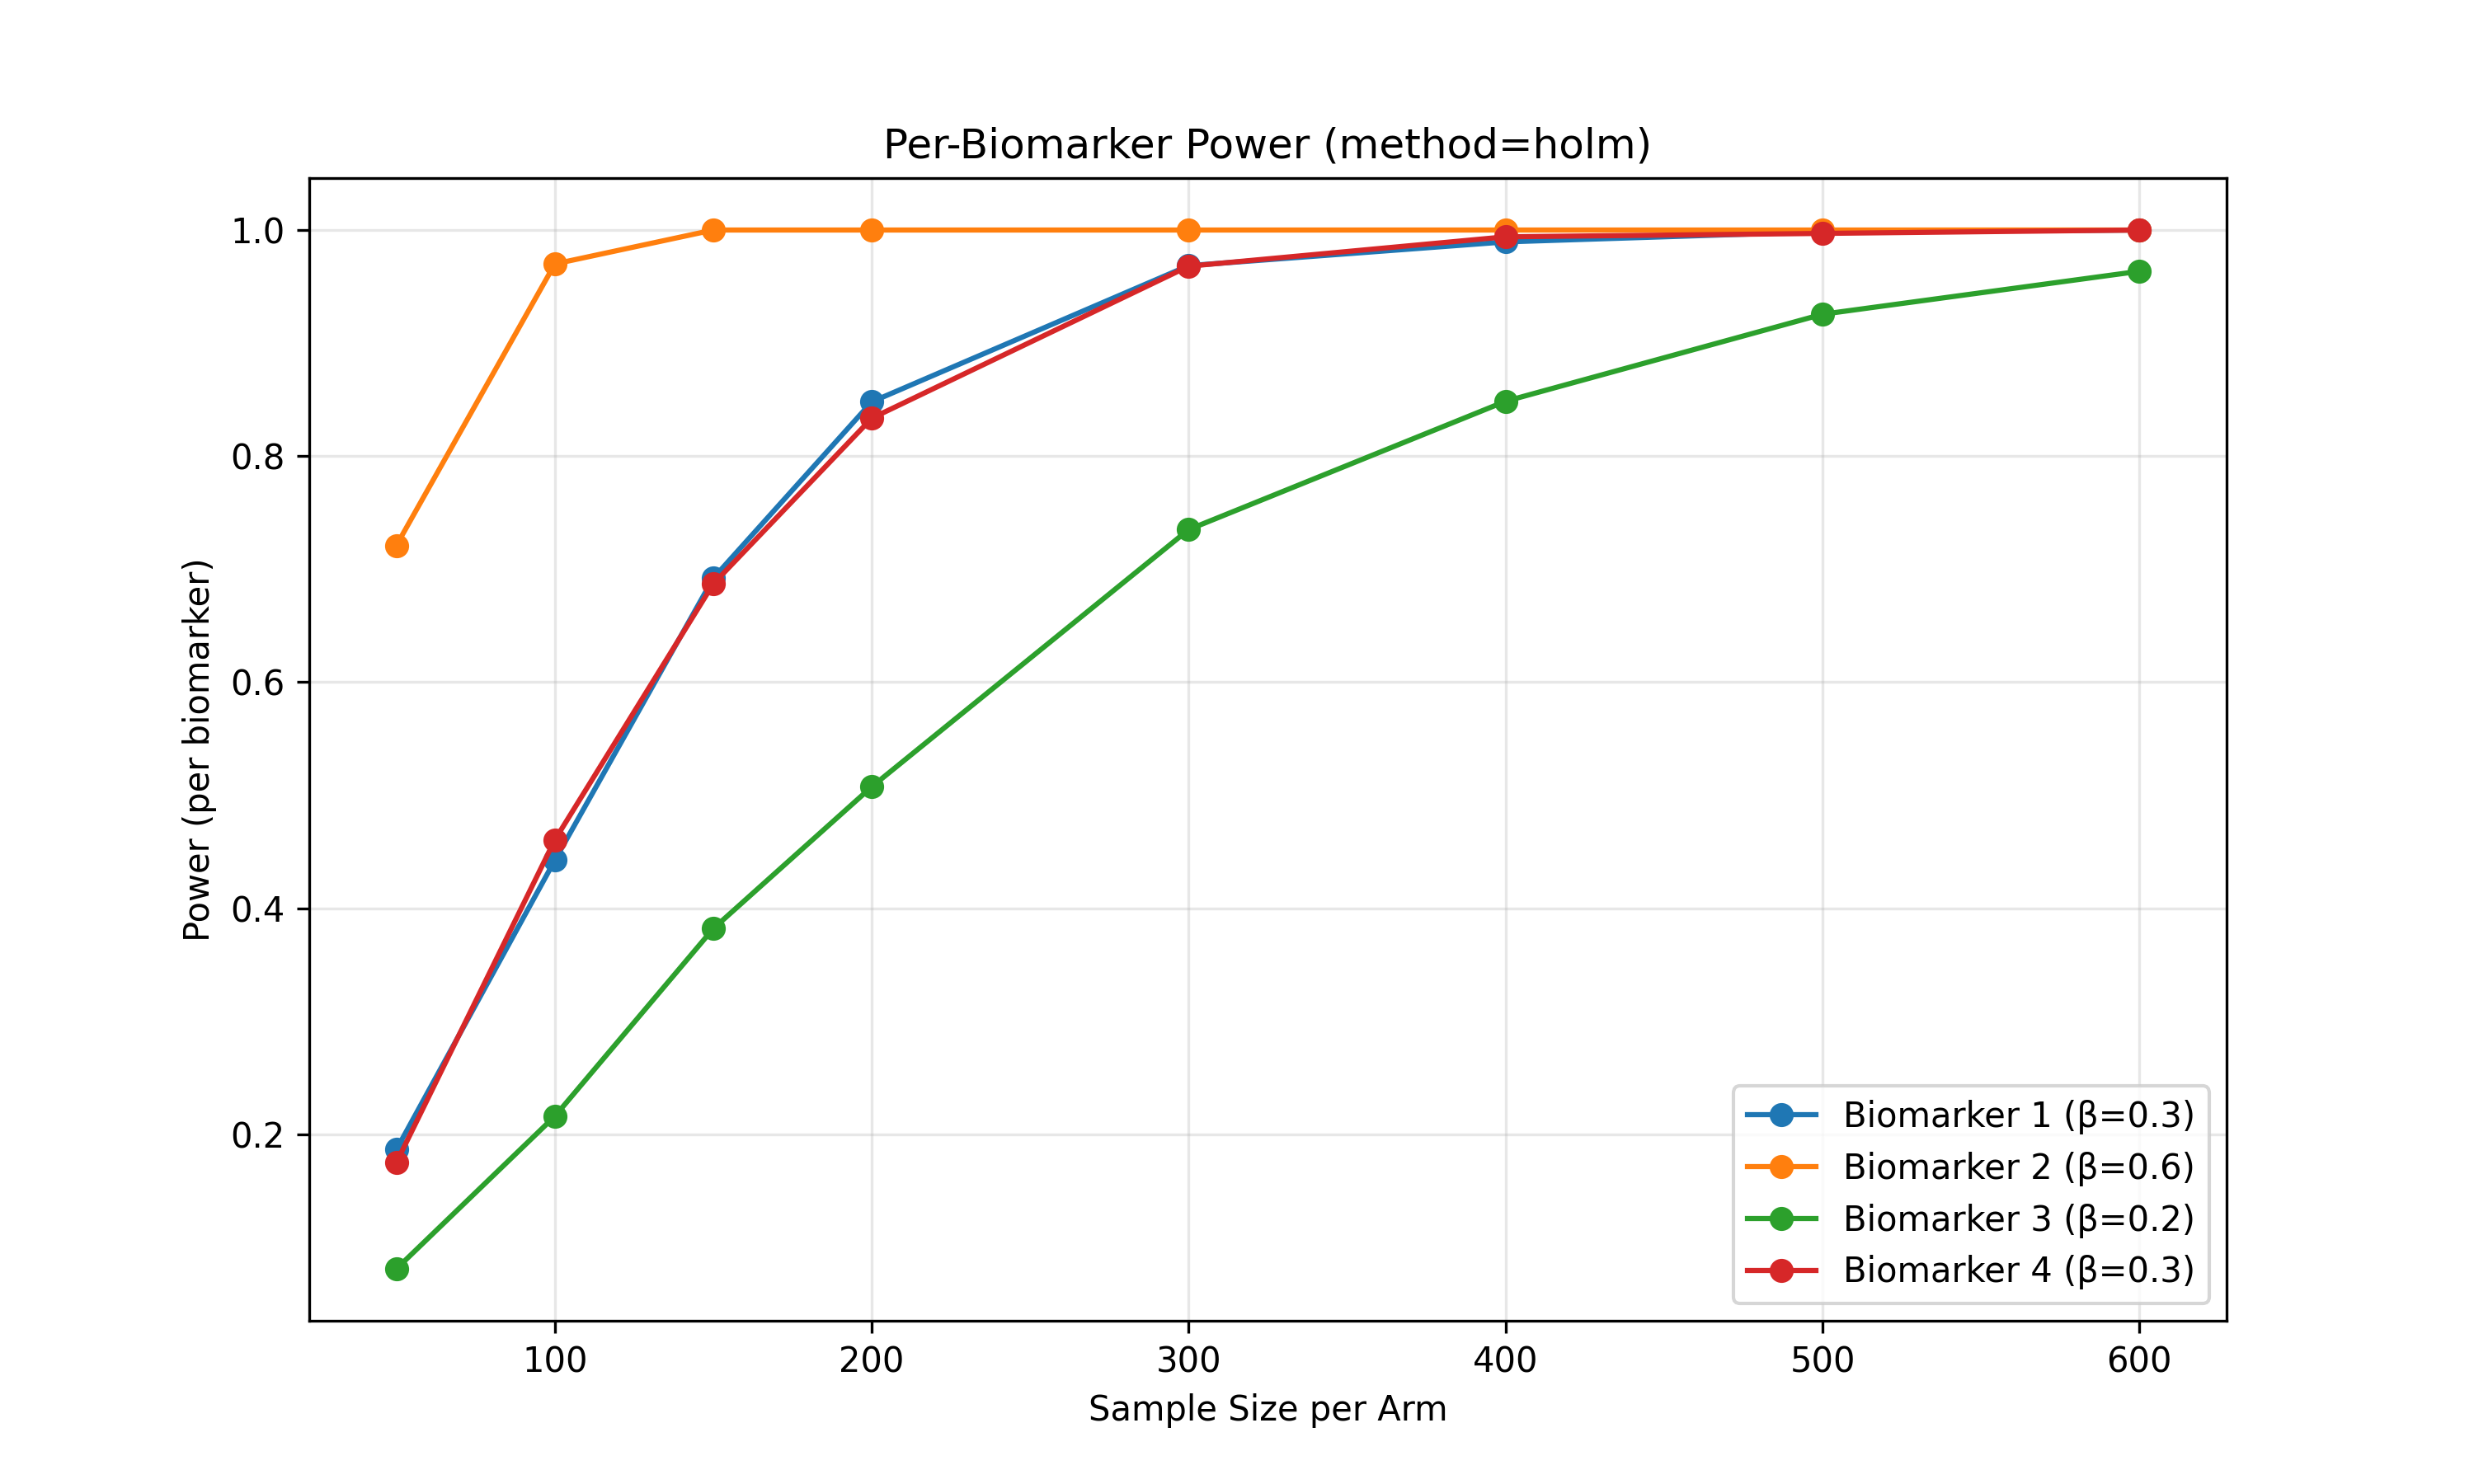
\includegraphics[width=1.0\textwidth]{figs/biomarker_power_holm.png}
\end{figure}

This figure shows the estimated statistical power for detecting each individual biomarker interaction (\(\beta_{3k}\)) plotted against the sample size {\it per arm} (assuming equal allocation to each arm), for $K=4$ arms. The figure shows that the required sample size is higher for smaller biomarker interaction sizes: A strong interaction (\(\beta_{3k}=0.60\)) with 80\% power takes 50 subjects in that arm, whereas a weak one (\(\beta_{3k} \approx 0.2\)) takes 350 subjects. If the trial's goal is to successfully validate \emph{all} $K$ biomarkers simultaneously, the overall sample size must be sufficient to detect the weakest hypothesized interaction at the desired power level; this model produces a total estimate of $n=1400$ subjects. We also assume the biomarkers themselves are correlated; the degree of this correlation further decreases power, necessitating even more samples. Estimating this correlation can also be done before beginning the trial, and would be worth doing.

\end{document} 